\documentclass[a4paper]{article}
\usepackage[english]{babel}
\usepackage{multicol}
\usepackage{amsmath}
\usepackage{amsfonts}
\usepackage{amssymb}
\usepackage[font=scriptsize]{caption}
\usepackage{parskip}
\usepackage[a4paper, margin=1in, total={6in, 8in}]{geometry}
\usepackage{titling}
\usepackage{subcaption}
\usepackage{float}
\usepackage{placeins}
\usepackage{graphicx}

\parskip = 6pt plus 2pt minus 2pt
\setlength{\droptitle}{-2cm}

\title{HW7 - Computer Simulation II}
\author{Schewtschik, Guilherme (3748052)}
\date{\today}

\begin{document}
\maketitle

\section{Cluster estimator for the correlation function}

For the 2D Ising model we compared the standard estimator
\[
G(R)=\langle s_i s_j\rangle
\]
with the cluster estimator
\[
\hat G(i,j)=\frac{V}{|C|}\Theta_C(i)\Theta_C(j),
\]
using the Wolff single-cluster algorithm for lattices of size
$L=64$ and $L=128$.

\begin{figure}[ht]
    \centering
    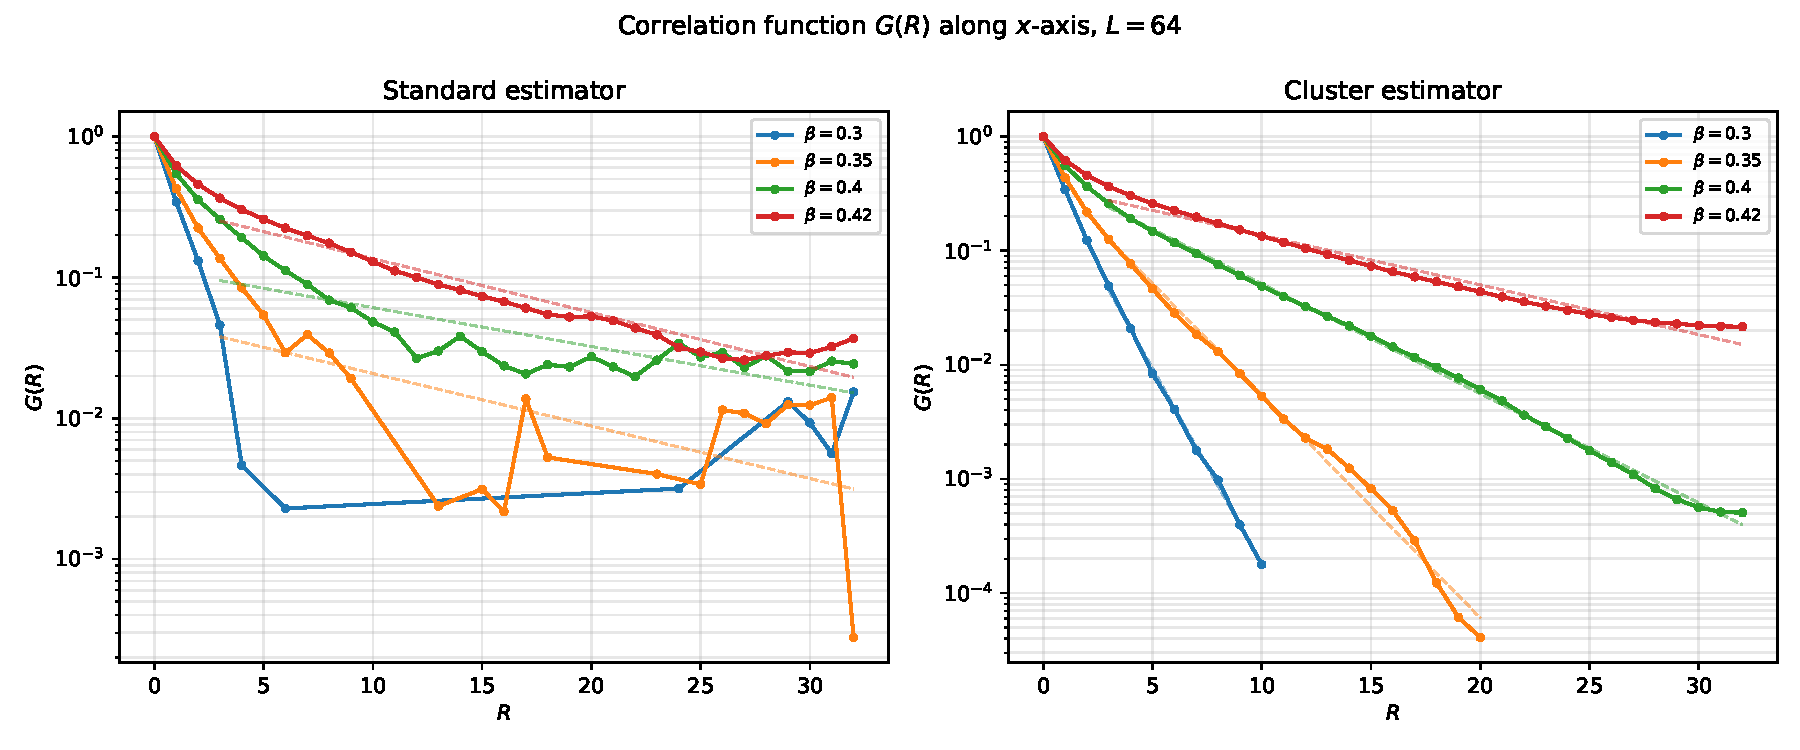
\includegraphics[width=0.7\linewidth]{figures/ising_correlation_G_L64.pdf}
    \caption{Correlation function $G(R)$ along the $x$-axis for $L=64$.}
\end{figure}

\begin{figure}[ht]
    \centering
    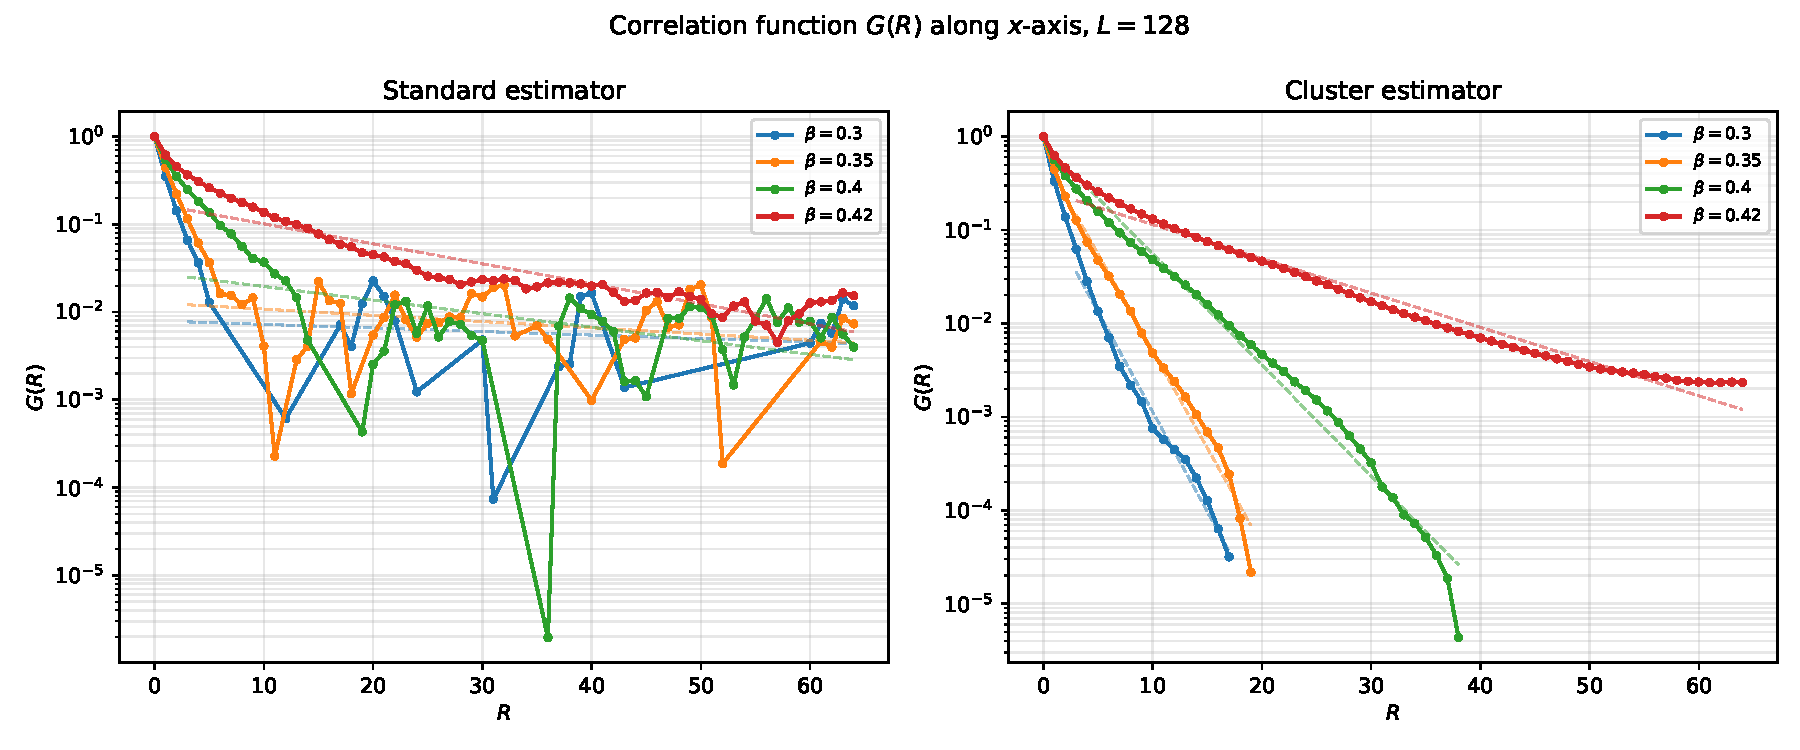
\includegraphics[width=0.7\linewidth]{figures/ising_correlation_G_L128.pdf}
    \caption{Correlation function $G(R)$ along the $x$-axis for $L=128$.}
\end{figure}

The correlation function decreases exponentially with distance for all
temperatures considered,
\[
G(R)\propto e^{-R/\xi}.
\]
The cluster estimator shows considerably smaller fluctuations than the
standard estimator, particularly at large distances where $G(R)$ is
small. This leads to a more accurate determination of the correlation
length.

\newpage

\begin{figure}[ht]
    \centering
    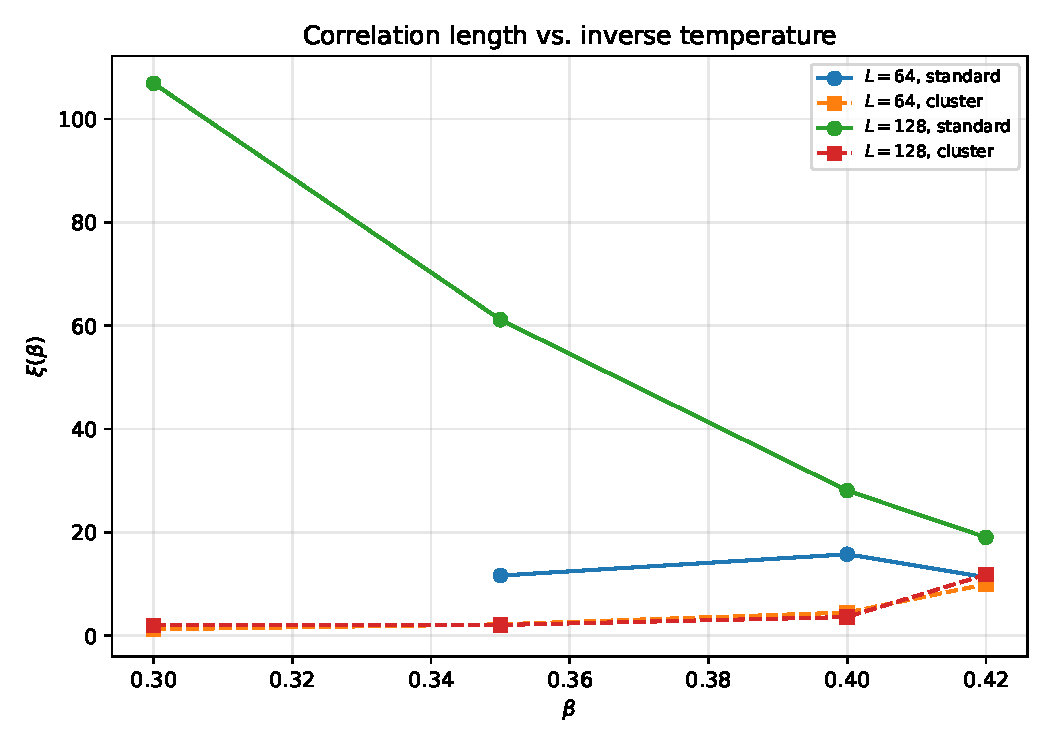
\includegraphics[width=0.6\linewidth]{figures/ising_xi_vs_beta.pdf}
    \caption{Correlation length as a function of inverse temperature.}
\end{figure}

As expected, the correlation length increases strongly with $\beta$ and
becomes largest close to the critical point. The results obtained for
$L=64$ and $L=128$ are consistent and indicate only small finite-size
effects in the investigated temperature range.


\section{Statistical error of histograms}

For a $16\times16$ lattice at $\beta_c\approx0.440686$,
the Metropolis algorithm was used with 5000 sweeps for thermalisation
and $2^{16}=65536$ sweeps for measurements.

\begin{figure}[ht]
    \centering
    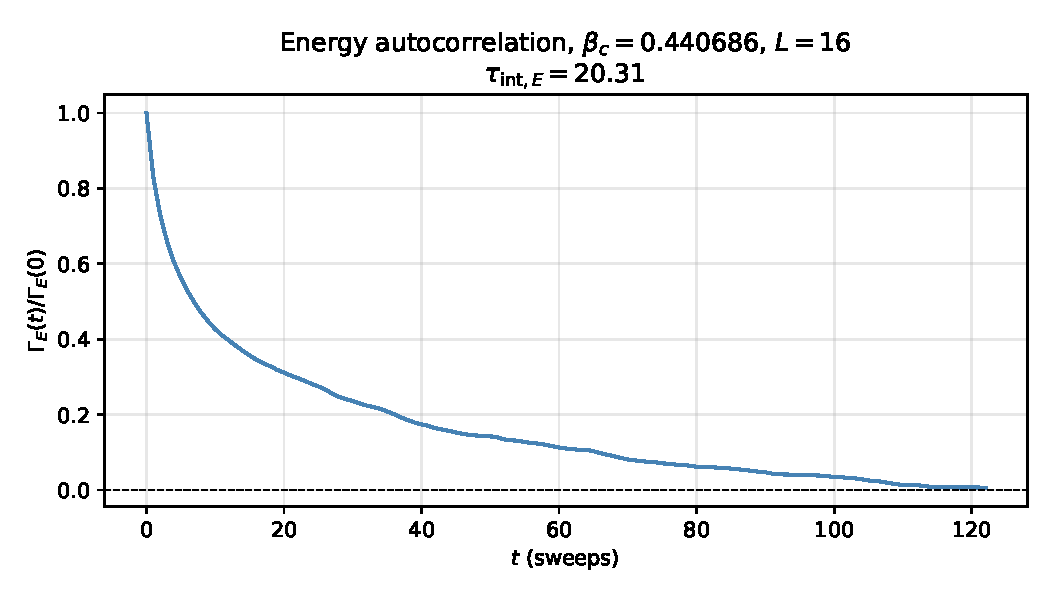
\includegraphics[width=0.7\linewidth]{figures/ising_autocorrelation_E.pdf}
    \caption{Energy autocorrelation function.}
\end{figure}

The integrated autocorrelation time obtained from the energy
autocorrelation function is
\[
\tau_{\mathrm{int},E}=20.31.
\]

\begin{figure}[ht]
    \centering
    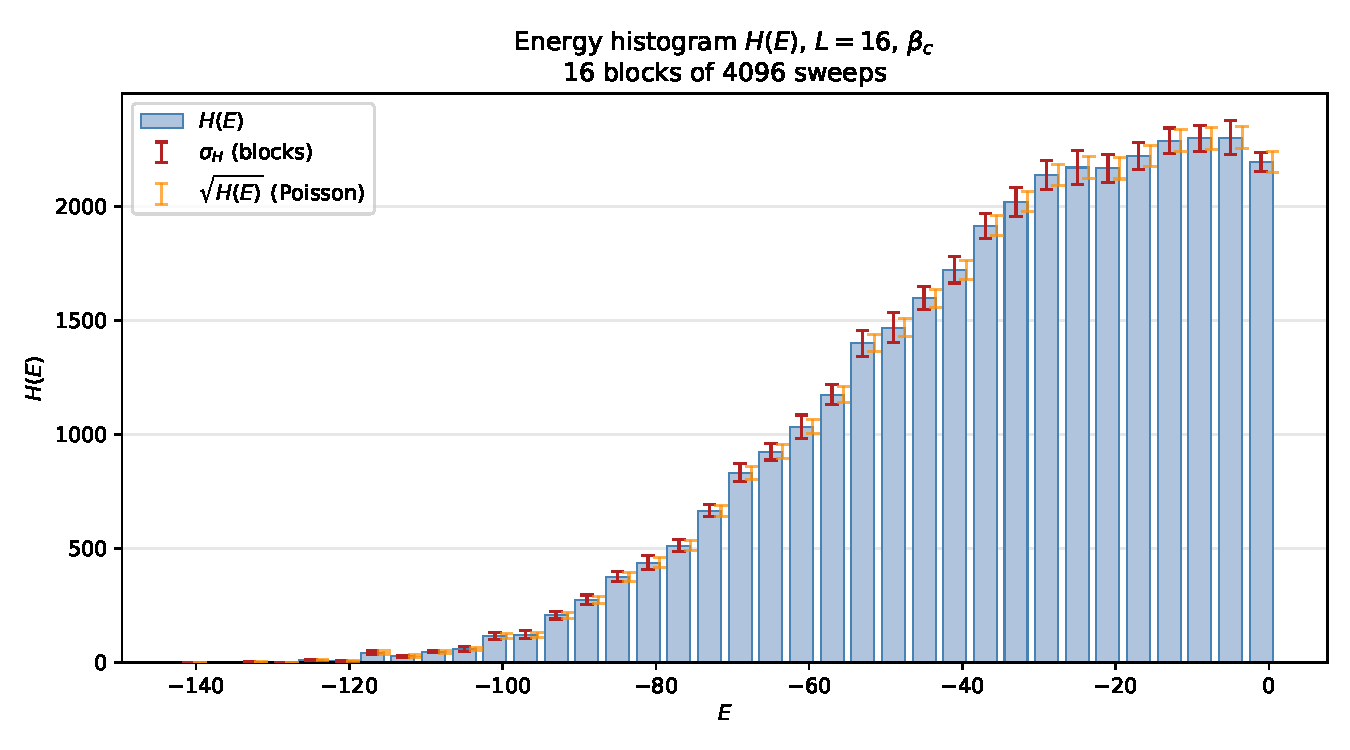
\includegraphics[width=0.7\linewidth]{figures/ising_histogram_E.pdf}
    \caption{Energy histogram $H(E)$.}
\end{figure}

The measured energy histogram agrees with the expected distribution at
criticality. The histogram errors were obtained from 16 blocks and
compared with the Poisson estimate
\[
\sigma_{H(E)}\simeq\sqrt{H(E)}.
\]

\begin{figure}[ht]
    \centering
    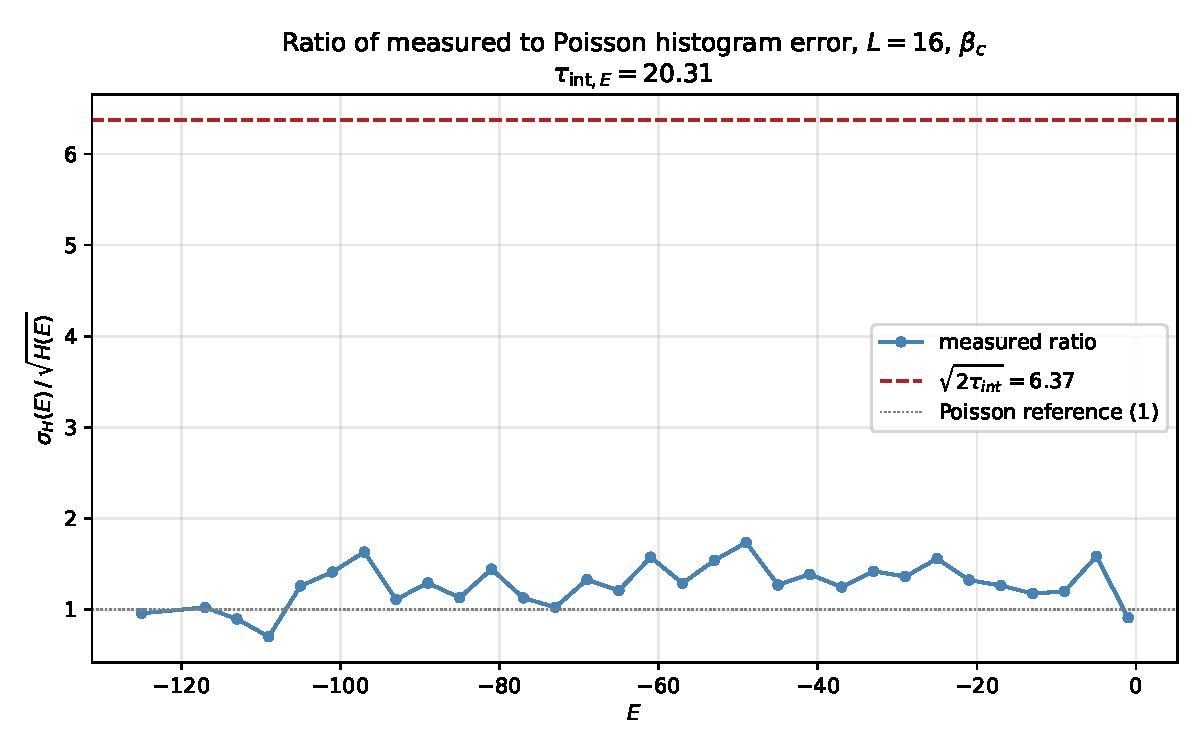
\includegraphics[width=0.7\linewidth]{figures/ising_histogram_ratio.pdf}
    \caption{Ratio of measured histogram error to the Poisson estimate.}
\end{figure}

The measured histogram errors are significantly larger than the Poisson
prediction due to autocorrelations in the Markov chain. From the
measured autocorrelation time we expect an enhancement factor
\[
\sqrt{2\tau_{\mathrm{int},E}}
=
\sqrt{2\cdot20.31}
=
6.37,
\]
which is consistent with the observed ratio. Therefore the histogram
errors are larger than $\sqrt{H(E)}$ by approximately the expected
factor arising from autocorrelated measurements.

\end{document}
